% sections/introduction.tex

\section{Introduction}
\label{sec:introduction}

The landscape of large language models has fragmented along multiple axes: modality (text, code, vision, diffusion), scale (1B to 1T+ parameters), cost (10$\times$ variation in per-token pricing), and specialization (general-purpose vs.\ domain-specific fine-tuning).
Organizations increasingly operate \emph{heterogeneous model fleets}---local vLLM instances alongside cloud endpoints from OpenAI, Anthropic, Azure, Bedrock, Gemini, and Vertex AI---each with different capabilities, pricing, and compliance characteristics.
This heterogeneity creates a fundamental inference-time optimization problem: \emph{given a user query, a fleet of diverse models, and deployment-specific constraints, which model should serve it, and what safety and privacy policies should apply?}

Viewed through the lens of information theory~\cite{shannon1948mathematical}, routing is an \emph{uncertainty-reduction} problem.
Before any analysis, routing entropy is maximal: $H(M \mid r_\text{raw}) \approx \log_2 K$ bits for $K$ candidate models---every model is equally plausible.
Each signal extracted from the request reduces this uncertainty.

The objective is to collapse $H(M \mid S(r))$ to near zero so the decision engine can make a deterministic, high-confidence routing choice (\Cref{fig:entropy_collapse}).
This viewpoint suggests a natural two-layer decomposition (\Cref{fig:shannon_mapping}).

In the first layer, signal extraction operates in the probabilistic regime of Shannon's \emph{Mathematical Theory of Communication}; in the second, decision evaluation operates in the algebraic regime of Shannon's \emph{switching-circuit algebra}~\cite{shannon1938symbolic}.
The signal vector~$\mathbf{s}$ is the interface between these regimes: continuous probabilistic inference below, discrete symbolic logic above.
In modern ML terms, the extraction layer behaves like a \emph{hybrid embedding stage} (\Cref{sec:disc_embedding}), while the priority-ordered decision engine behaves like a \emph{symbolic Mixture-of-Experts gate} with deterministic early exit (\Cref{sec:disc_moe}).
We further view priority blocks as \emph{layered entropy folding} (\Cref{sec:disc_entropy_folding}), yielding a programmable neural-symbolic inference engine (Transformer-like control structure but not equivalent hidden-state dynamics) that we connect to agent-based policy synthesis (\Cref{sec:disc_agent}).

\begin{figure*}[!ht]
  \centering
  \resizebox{\linewidth}{!}{%
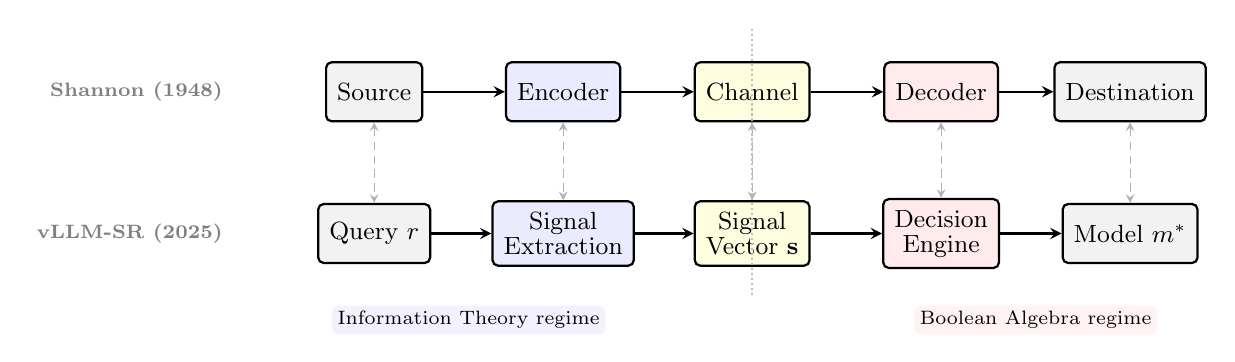
\begin{tikzpicture}[
    sbox/.style={rectangle, draw, thick, rounded corners=2pt,
                 minimum height=0.75cm, align=center, inner sep=4pt, font=\small},
    lbl/.style={font=\scriptsize, text=gray},
    arr/.style={->, >=stealth, thick},
    darr/.style={<->, >=stealth, densely dashed, gray!60, thin},
  ]

  % --- Shannon row (top) ---
  \node[lbl, anchor=east] at (-0.6, 1.8) {\textbf{Shannon (1948)}};
  \node[sbox, fill=black!5]  (src)  at (1.2, 1.8) {Source};
  \node[sbox, fill=blue!8]   (senc) at (3.6, 1.8) {Encoder};
  \node[sbox, fill=yellow!12] (ch)  at (6.0, 1.8) {Channel};
  \node[sbox, fill=red!8]    (sdec) at (8.4, 1.8) {Decoder};
  \node[sbox, fill=black!5]  (dst)  at (10.8, 1.8) {Destination};

  \draw[arr] (src) -- (senc);
  \draw[arr] (senc) -- (ch);
  \draw[arr] (ch) -- (sdec);
  \draw[arr] (sdec) -- (dst);

  % --- VSR row (bottom) ---
  \node[lbl, anchor=east] at (-0.6, 0) {\textbf{vLLM-SR (2025)}};
  \node[sbox, fill=black!5]  (qry) at (1.2, 0) {Query $r$};
  \node[sbox, fill=blue!8]   (sig) at (3.6, 0) {Signal\\[-2pt]Extraction};
  \node[sbox, fill=yellow!12] (sv)  at (6.0, 0) {Signal\\[-2pt]Vector $\mathbf{s}$};
  \node[sbox, fill=red!8]    (dec) at (8.4, 0) {Decision\\[-2pt]Engine};
  \node[sbox, fill=black!5]  (mdl) at (10.8, 0) {Model $m^*$};

  \draw[arr] (qry) -- (sig);
  \draw[arr] (sig) -- (sv);
  \draw[arr] (sv) -- (dec);
  \draw[arr] (dec) -- (mdl);

  % --- Correspondence arrows ---
  \draw[darr] (src.south)  -- (qry.north);
  \draw[darr] (senc.south) -- (sig.north);
  \draw[darr] (ch.south)   -- (sv.north);
  \draw[darr] (sdec.south) -- (dec.north);
  \draw[darr] (dst.south)  -- (mdl.north);

  % --- Regime labels ---
  \draw[densely dotted, gray!50, thick] (6.0, 2.6) -- (6.0, -0.8);
  \node[font=\scriptsize, fill=blue!5, rounded corners=2pt, inner sep=2pt]
    at (2.4, -1.1) {Information Theory regime};
  \node[font=\scriptsize, fill=red!5, rounded corners=2pt, inner sep=2pt]
    at (9.6, -1.1) {Boolean Algebra regime};

  \end{tikzpicture}%
}
  \caption{Structural correspondence between Shannon's communication system~\cite{shannon1948mathematical} and VSR's routing pipeline.
  The dotted line marks the boundary between the information-theoretic regime (signal extraction maximizes mutual information with the routing outcome) and the Boolean-algebraic regime (the decision engine synthesizes routing policies from signal conditions via $\{\wedge, \vee, \neg\}$~\cite{shannon1938symbolic}).}
  \label{fig:shannon_mapping}
\end{figure*}

\begin{figure*}[!ht]
  \centering
  \resizebox{\linewidth}{!}{%
\begin{tikzpicture}[
    bar/.style={draw, thick, rounded corners=1pt, fill=#1, minimum width=0.9cm, anchor=south},
    lbl/.style={font=\scriptsize},
    arr/.style={->, >=stealth, thick, gray!70},
  ]

  % Bars (heights represent entropy)
  \node[bar=gray!20,   minimum height=3.2cm] (b0) at (0.8, 0) {};
  \node[bar=blue!15,   minimum height=2.4cm] (b1) at (2.4, 0) {};
  \node[bar=blue!20,   minimum height=1.6cm] (b2) at (4.0, 0) {};
  \node[bar=blue!25,   minimum height=0.9cm] (b3) at (5.6, 0) {};
  \node[bar=green!20,  minimum height=0.2cm] (b4) at (7.2, 0) {};

  % Bar labels (top)
  \node[lbl, above=1pt of b0] {$\log_2 K$};
  \node[lbl, above=1pt of b1] {};
  \node[lbl, above=1pt of b2] {};
  \node[lbl, above=1pt of b3] {};
  \node[lbl, above=1pt of b4] {$\approx 0$};

  % Bar labels (bottom)
  \node[lbl, below=2pt of b0, align=center] {Raw\\[-1pt]query};
  \node[lbl, below=2pt of b1, align=center] {+keyword\\[-1pt]+language};
  \node[lbl, below=2pt of b2, align=center] {+domain};
  \node[lbl, below=2pt of b3, align=center] {+complexity\\[-1pt]+embedding};
  \node[lbl, below=2pt of b4, align=center] {Decision\\[-1pt]$\phi(\mathbf{s})$};

  % Arrows between bars
  \draw[arr] (b0.east) -- (b1.west);
  \draw[arr] (b1.east) -- (b2.west);
  \draw[arr] (b2.east) -- (b3.west);
  \draw[arr] (b3.east) -- (b4.west);

  % Y-axis label
  \node[font=\scriptsize, rotate=90, anchor=south] at (-0.2, 1.6) {$H(M \mid \text{signals observed})$};

  % Baseline
  \draw[gray!40] (-0.1, 0) -- (8.0, 0);

  \end{tikzpicture}%
}
  \caption{Entropy collapse during signal extraction. Each additional signal reduces the routing uncertainty $H(M \mid \cdot\,)$ from the uniform prior $\log_2 K$ bits until the decision formula $\phi(\mathbf{s})$ yields a near-deterministic model selection.}
  \label{fig:entropy_collapse}
\end{figure*}

This problem is more nuanced than binary difficulty routing.
A production routing system must simultaneously consider:
\begin{itemize}[leftmargin=*]
  \item \textbf{Multi-dimensional signals}: Query domain, modality, complexity, language, user identity, and real-time performance metrics all inform the optimal routing decision.
  \item \textbf{Privacy and safety}: Prompt injection, PII leakage, and hallucinated responses must be detected and mitigated---often with \emph{different policies for different query types and user roles}.
  \item \textbf{Cost-effective model selection}: Algorithms must balance response quality against inference cost and latency, selecting from a heterogeneous pool of local and cloud-hosted models.
  \item \textbf{Deployment diversity}: The same routing framework must serve a privacy-regulated healthcare deployment (strict PII filtering, on-premise models only), a cost-optimized developer tool (aggressive caching, cheapest model first), and a multi-cloud enterprise (failover across providers)---through configuration, not code changes.
  \item \textbf{Multi-turn statefulness}: Routing decisions must be consistent across conversation turns, requiring stateful session management and context preservation.
\end{itemize}

Prior work on LLM routing has made significant progress on individual aspects.
RouteLLM~\cite{ong2024routellm} trains classifiers to route between two models based on query difficulty.
RouterDC~\cite{chen2024routerdc} learns query-model embeddings via dual contrastive learning.
AutoMix~\cite{aggarwal2023automix} formulates cascading as a POMDP.
However, these approaches address model selection in isolation, without integrating signal extraction, safety enforcement, multi-provider backend management, or plugin extensibility into a unified framework.

\subsection{Contributions}

We present \sysname{}, a signal-driven decision routing system whose central innovation is \textbf{composable signal orchestration}: heterogeneous signals are extracted, composed through Boolean rules into deployment-specific decisions, and executed through per-decision plugin chains---enabling a single architecture to serve diverse deployment scenarios.

Our contributions are:

\begin{enumerate}[leftmargin=*]
  \item \textbf{Composable Signal-Decision-Plugin Architecture} (\Cref{sec:architecture,sec:signal_engine,sec:decision_engine,sec:plugins}):
    A three-layer architecture where thirteen signal types are composed through Boolean decision rules into deployment-specific routing policies, with per-decision plugin chains for safety, caching, and augmentation. Different deployment scenarios (privacy-regulated, cost-optimized, multi-cloud) are expressed as different configurations over the same architecture.

  \item \textbf{Semantic Model Routing with Cost-Aware Selection} (\Cref{sec:model_selection}):
    A unified framework integrating thirteen model selection algorithms---rating-based, contrastive, cascading, classical ML, reinforcement learning, and latency-aware---that analyze request semantics to select the most cost-effective model while respecting per-decision privacy and safety constraints.

  \item \textbf{HaluGate: Gated Hallucination Detection} (\Cref{sec:halugate}):
    A three-stage pipeline---sentinel gating, token-level detection, NLI-based explanation---that avoids unnecessary verification on non-factual queries while providing span-level diagnostics when hallucination is detected.

  \item \textbf{Multi-Provider and Multi-Endpoint Routing} (\Cref{sec:extproc}):
    Native support for routing across heterogeneous backends (vLLM, OpenAI, Anthropic, Azure, Bedrock, Gemini, Vertex AI) with provider-specific protocol translation, a pluggable authorization factory for diverse auth mechanisms, weighted multi-endpoint load distribution, and full OpenAI Responses API support for stateful multi-turn conversations.

  \item \textbf{LoRA-Based Multi-Task Classification} (\Cref{sec:lora_mom,sec:ml_inference}):
    A memory-efficient architecture using Low-Rank Adaptation that serves $n$ classification tasks from a single base model with lightweight adapter heads, reducing aggregate model memory from $n$ full copies to one base plus negligible adapter overhead.

  \item \textbf{Episodic Conversation Memory with ReflectionGate} (\Cref{sec:memory_rag}):
    A lightweight memory system that stores raw conversational turns as episodic chunks (filtered by an entropy gate and capped at 16\,KB) rather than relying on LLM-based fact extraction, eliminating inference overhead at write time.
    At retrieval time, a multi-stage \emph{ReflectionGate} pipeline---safety block-pattern filtering, recency decay, Jaccard deduplication, and budget capping---refines retrieved chunks before injection as a separate context message, enabling personalized multi-turn routing without coupling memory quality to an external model.

  \item \textbf{Programmable Neural-Symbolic Configuration Language} (\Cref{sec:dsl}):
    A typed configuration language that serves as the instruction set of the routing inference engine, with a formal grammar parsed into a Boolean expression AST, three-level validation (syntax, reference, constraint), multi-target compilation (flat YAML, Kubernetes CRDs, Helm charts), and round-trip decompilation.
    We formalize the system as a \emph{programmable neural-symbolic inference engine}---neural signal extraction as a hybrid embedding layer, symbolic decision evaluation as Mixture-of-Experts gating---and show that the language's functional completeness enables LLM-based coding agents to synthesize routing policies from natural-language specifications.
\end{enumerate}

\subsection{Paper Organization}

\Cref{sec:architecture} presents the system architecture and composable orchestration model.
\Cref{sec:signal_engine,sec:decision_engine} formalize the signal extraction and decision evaluation layers.
\Cref{sec:plugins,sec:safety,sec:halugate} describe the plugin framework and safety subsystems.
\Cref{sec:lora_mom,sec:ml_inference} detail the LoRA-based classification architecture and multi-runtime inference design.
\Cref{sec:model_selection} surveys the semantic model selection algorithms.
\Cref{sec:extproc} describes the multi-provider request processing pipeline.
\Cref{sec:memory_rag,sec:observability,sec:deployment} cover memory, observability, and deployment.
\Cref{sec:evaluation} presents evaluation results.
\Cref{sec:dsl} specifies the programmable configuration language and develops the neural-symbolic inference engine perspective.
\Cref{sec:related_work} discusses related work, and \Cref{sec:conclusion} concludes.
